\section{Demonstration Scenario}
\label{sec:demo}
The demonstration uses a synthetic panel with an explicitly specified requirement: after \texttt{close}, work started in the previous epoch must not publish. The example isolates this requirement; it is not an independently collected repository incident. Listing~\ref{lst:panel} shows the protected version. Removing the capture of \texttt{started} and its comparison yields the unguarded version. The epoch protection is supplied by the reviewer.

\begin{lstlisting}[language=JavaScript,caption={Protected synthetic panel; the requirement is supplied with the example.},label={lst:panel}]
function createPanel(fetchValue, publish) {
  let epoch = 0;
  async function refresh() {
    const started = epoch;
    const value = await fetchValue();
    if (started !== epoch) return;
    publish(value);
  }
  function close() { epoch += 1; }
  return {refresh, close};
}
\end{lstlisting}

\paragraph{Locate and inspect.}
The presenter scans the unguarded version and opens its archived report. Three rules identify an effect after a wait, a continuation near a lifecycle boundary, and guard-state review. The first links the wait to the later \texttt{publish} call in source order. The lifecycle cards nominate the nearby close operation and state update. Their references support investigation; the presenter still checks that the returned operations share the panel's lexical state.

\begin{figure*}[t]
\centering
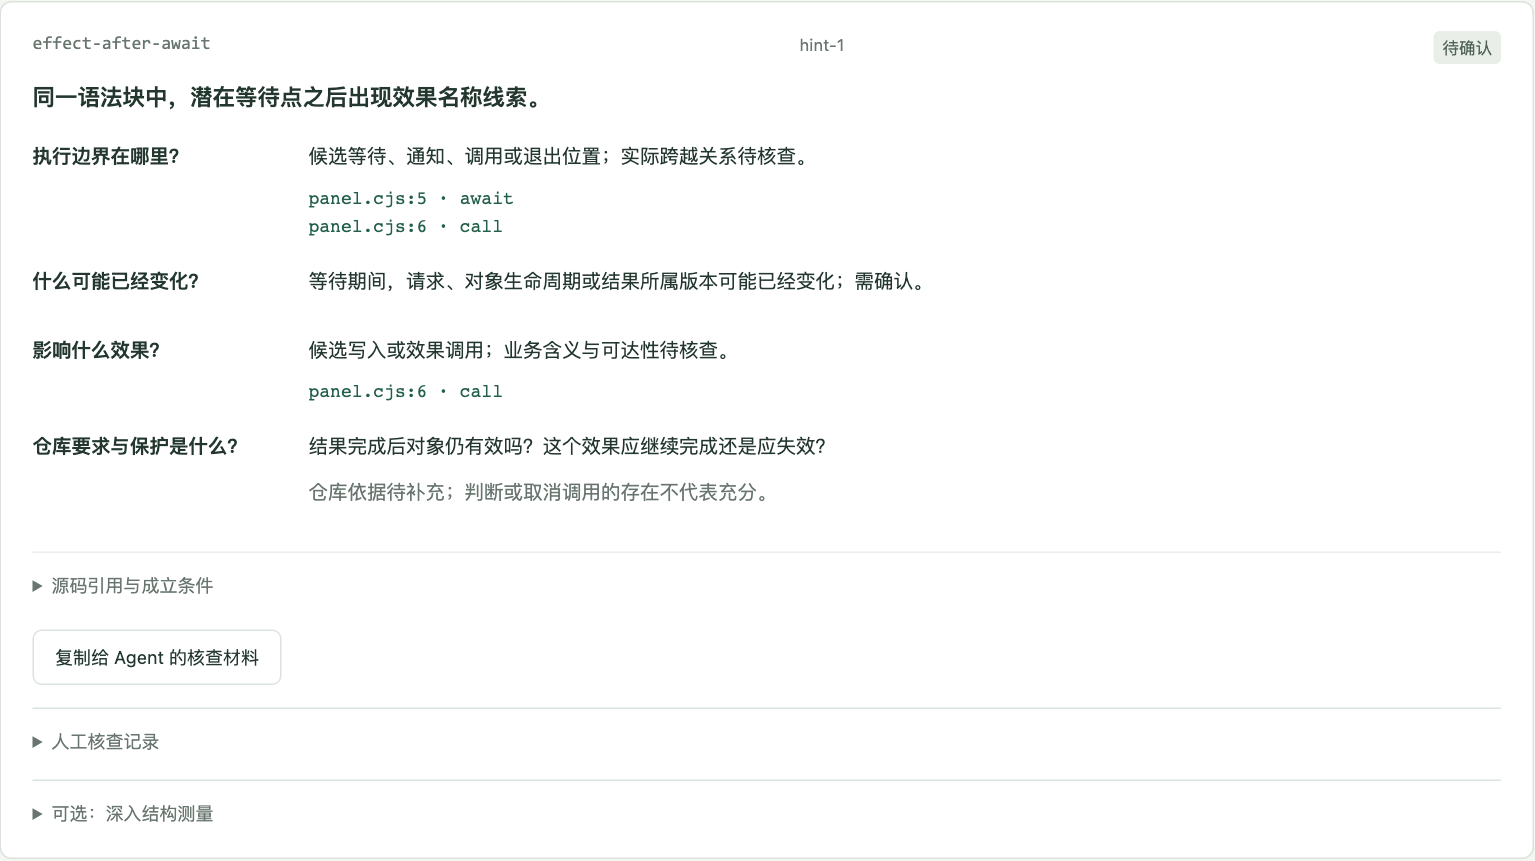
\includegraphics[width=0.90\textwidth]{figures/workbench.png}
\caption{Actual review card for the synthetic unguarded panel. The current interface uses Chinese labels; the four fields correspond to boundary, possible change, affected effects, and requirement/protection. Source references open the archived evidence.}
\label{fig:workbench}
\end{figure*}

\paragraph{Establish behavior.}
A separate replay script starts \texttt{refresh}, calls \texttt{close}, resolves the pending request, and awaits the continuation. The unguarded version publishes \texttt{old result}; the protected version produces no publication. This script executes the paper's synthetic programs independently of scanning. The observed behavior witnesses this particular schedule and stated requirement.

\paragraph{Review the protection.}
The presenter inspects the epoch comparison and records relation validity separately from protection sufficiency. The supplied capture script also saves an author-demonstration annotation for the unguarded report; this is a walkthrough record, not an independent judgment. Both versions retain the same three rule kinds. In the protected version, the guard-state card also references the conditional guard. The reviewer must determine why that guard connects the continuing work to its initiating epoch. A reduction in hint count would miss the relevant difference.

The session ends by comparing the archived versions. The comparison reports a changed guard-evidence finding while the rule kinds and total count stay constant. Reading either report through MCP retrieves that version's frozen materials; annotation history remains available in the workbench. The replay supplies the separate behavioral witness.
